\documentclass[border=4pt]{standalone}
\usepackage{times,amsmath}
\usepackage[T1]{fontenc}
\usepackage{tikz}
\usetikzlibrary{patterns,arrows.meta,calc,decorations.markings}
\definecolor{lone}{RGB}{31,119,180}
\definecolor{ltwo}{RGB}{230,97,0}
\definecolor{tauc}{RGB}{200,30,30}
\begin{document}
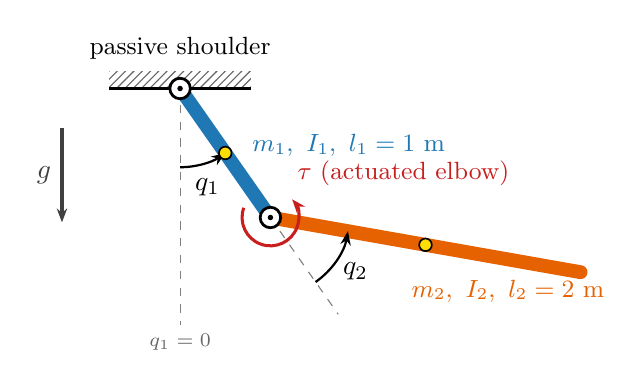
\begin{tikzpicture}[scale=1.0, >={Stealth[length=5pt]}]
  \def\La{2.0}  % l1 = 1 m
  \def\Lb{4.0}  % l2 = 2 m
  \def\qa{35}   % q1
  \def\qb{45}   % q2
  \coordinate (O) at (0,0);
  \coordinate (E) at ({-90+\qa}:\La);
  \coordinate (T) at ($(E)+({-90+\qa+\qb}:\Lb)$);
  \coordinate (C1) at ({-90+\qa}:\La/2);
  \coordinate (C2) at ($(E)+({-90+\qa+\qb}:\Lb/2)$);
  % ceiling
  \fill[pattern=north east lines, pattern color=black!60] (-0.9,0) rectangle (0.9,0.22);
  \draw[line width=0.9pt] (-0.9,0) -- (0.9,0);
  % reference lines
  \draw[dashed, black!50] (O) -- (0,-3.0);
  \draw[dashed, black!50] (E) -- ($(E)+({-90+\qa}:1.5)$);
  % links
  \draw[line width=5pt, lone, line cap=round] (O) -- (E);
  \draw[line width=5pt, ltwo, line cap=round] (E) -- (T);
  % angles
  \draw[->, thick] (0,-1.0) arc[start angle=-90, end angle={-90+\qa}, radius=1.0];
  \node at ({-90+\qa/2-2}:1.3) {$q_1$};
  \draw[->, thick] ($(E)+({-90+\qa}:1.0)$) arc[start angle={-90+\qa}, end angle={-90+\qa+\qb}, radius=1.0];
  \node at ($(E)+({-90+\qa+\qb/2}:1.28)$) {$q_2$};
  % torque
  \draw[->, tauc, line width=1.1pt] ($(E)+(160:0.36)$) arc[start angle=160, end angle=400, radius=0.36];
  \node[tauc, anchor=south west, font=\small] at ($(E)+(0.22,0.28)$) {$\tau$ (actuated elbow)};
  % joints
  \draw[fill=white, line width=1pt] (O) circle (0.13); \fill (O) circle (0.035);
  \draw[fill=white, line width=1pt] (E) circle (0.13); \fill (E) circle (0.035);
  % COMs
  \foreach \c in {C1,C2} {\draw[fill=yellow!80!orange, line width=0.6pt] (\c) circle (0.08);}
  % labels
  \node[anchor=south] at (0,0.25) {\small passive shoulder};
  \node[lone, anchor=west, font=\small] at ($(C1)+(0.22,0.1)$) {$m_1,\ I_1,\ l_1 = 1$ m};
  \node[ltwo, anchor=north west, font=\small] at ($(C2)+(-0.3,-0.32)$) {$m_2,\ I_2,\ l_2 = 2$ m};
  % gravity
  \draw[->, line width=1.2pt, black!75] (-1.5,-0.5) -- (-1.5,-1.7) node[midway, left] {$g$};
  \node[font=\scriptsize, black!60, anchor=north] at (0,-3.0) {$q_1 = 0$};
\end{tikzpicture}
\end{document}
